%%%%%%%%%%%%%%%%%%%%%%%%%%%%%%%%%%%%%%%%%
% University/School Laboratory Report
% LaTeX Template
% Version 4.0 (March 21, 2022)
%
% This template originates from:
% https://www.LaTeXTemplates.com
%
% Authors:
% Vel (vel@latextemplates.com)
% Linux and Unix Users Group at Virginia Tech Wiki
%
% License:
% CC BY-NC-SA 4.0 (https://creativecommons.org/licenses/by-nc-sa/4.0/)
%
%%%%%%%%%%%%%%%%%%%%%%%%%%%%%%%%%%%%%%%%%

%----------------------------------------------------------------------------------------
%	PACKAGES AND DOCUMENT CONFIGURATIONS
%----------------------------------------------------------------------------------------

\documentclass[
	article, % Paper size, specify a4paper (A4) or letterpaper (US letter)
	11pt, % Default font size, specify 10pt, 11pt or 12pt
]{CSUniSchoolLabReport}


\addbibresource{reference.bib} % Bibliography file (located in the same folder as the template)

\usepackage{enumitem}
\usepackage{hyperref}

%----------------------------------------------------------------------------------------
%	REPORT INFORMATION
%----------------------------------------------------------------------------------------

\title{CSC3105 Data Analytics Assignment} % Report title

\author{
        Woon Jun Wei \textit{2200624} \\
        Benjamin Loh Choon How \textit{2201590} \\
        Low Hong Sheng Jovian \textit{2203654}\\
        Wang Rongqi Richie \textit{2201942} \\
        Poon Xiang Yuan \textit{2200559} \\
    }

\date{\today} % Date of the report

%----------------------------------------------------------------------------------------

\begin{document}

\maketitle % Insert the title, author and date using the information specified above



% START of Jovian's draft for JW's verdict ): %
% DON TOUCH HERE unless u want to add on stuff %
\section{Background}\label{background}

\subsection{Emergence of IoT and Indoor Positioning Needs}\label{Emergence of IoT and Indoor Positioning Needs}
The advent of the Internet of Things (IoT) has revolutionized how we interact with our environment, giving rise to an increased demand for precise Indoor Positioning Systems (IPS). Applications range from pedestrian tracking to autonomous drones in logistics and social distancing protocols, all requiring reliable localization technologies.

\subsection{Limitations of GNSS in Indoor Environments}\label{Limitations of GNSS in Indoor Environments}
While the Global Navigation Satelite System (GNSS) has been a cornerstone for ourdoor localization, its effectiveness is drastically reduced indoors due to signal attentuation by obstacles like walls, making it unsuitable for indoor use.

\subsection{The Promise of UWB Technology}\label{The Promise of UWB Technology}
Ultra-Wideband (UWB) technology, with its short pulse duration, offers high temporal resolution, enabling high accuracy in IPS. Nonetheless, the accuracy of Ultra-wideband (UWB) systems is compromised under Non-Line-Of-Sight (NLOS) conditions, where signal obstructions or reflections occur, presenting a substantial hurdle due to the resulting deterioration in localization precision.

\subsection{Current NLOS Identification Methods}\label{Current NLOS Identification Methods}
The academic and industrial sectors have explored numerous methodologies to mitigate the NLOS issue in UWB systems. These range from non-feature-based approaches, leveraging contextual information, to feature-based methods that extract distinct waveform characteristics to identify NLOS conditions using maching learning (ML) techniques.

\subsection{Challenges and Limitations}\label{Challenges and Limitations}
Although ML has emerged as a promising solution for NLOS identification, existing feature-based approaches face challenges, particularly with imbalanced datasets where NLOS samples are scarce. This affects the robustness of the classifiers being trained.

\section{Introduction to the Project}\label{Introduction to the Project}
Against this backdrop, our project aims to address the critical challenge of distinguishing between LOS and NLOS conditions in UWB-based IPS. We intend to train a machine learning model using the given dataset, with the ultimate goal of enhancing UWB localization accuracy irrespective of LOS or NLOS conditions. Acknowledging the limitations of traditional ML approaches in handling imbalanced data, we will explore a three-dimensional-process-centric approach over sheer accuracy metrics. This strategy focuses on developing a robust classifier that remains effective even with limited NLOS data, a common scenario in real-world applications.


% og intro, if above ok can combine / remove %
\section{Introduction}\label{introduction}
In the realm of signal processing and analytics, a diverse array of operations is available for data preprocessing, model training (data mining), and visualization. Notably, signal data acquired from Ultra-Wideband (UWB) Internet of Things (IoT) sensors often exhibits inherent inaccuracies and susceptibility to noise and interference.

\cite{jiang_uwb_2020} introduced a novel methodology for data preprocessing and denoising in their seminal work. Moreover, they advocated for the utilization of sophisticated unsupervised machine learning algorithms, including Support Vector Machines (SVM), Convolutional Neural Networks (CNN), and Multilayer Perceptrons (MLP), for modeling the intricate dynamics of the acquired data.

Their pioneering approach not only addresses the challenges associated with noisy UWB IoT sensor data but also underscores the efficacy of employing advanced machine learning techniques for insightful data analysis and interpretation.

An approach to calculate distance, as introduced by \cite{che_feature-based_2022}, involves leveraging Time-Of-Arrival (TOA) and Trilateration methodologies. However, due to the absence of detailed anchorpoint information, the Trilateration approach could not be executed. Instead, a modified formula was employed:


\begin{equation}
\text{Total Distance} = \sum_{i=1}^{n} |CIR_i| \cdot c
\end{equation}

where:

\begin{itemize}
  \item $CIR_i$ represents the Channel Impulse Response for the $i$-th anchor point.
  \item $c$ is the speed of light in a vacuum, approximately $2.99792458 \times 10^8 \text{ m/s}$. We can use a constant value here for simplicity, assuming the context focuses on light propagation.
\end{itemize}

This formula facilitates distance estimation based on the cumulative Channel Impulse Response and the speed of light in nanoseconds. However, it's noteworthy that this derived feature is not utilized as part of the data mining process.



\subsection{Objective}\label{objective}

The primary aim of this assignment is to develop a model capable of discerning whether a given set of Channel Impulse Response (CIR) measurements corresponds to Line-of-Sight (LOS) or Non-Line-of-Sight (NLOS) scenarios. This entails the comprehensive execution of the three-dimensional process, encompassing Data Preprocessing, Data Mining, and Data Visualization. By diligently executing each phase of this process, the objective is to achieve a robust and insightful understanding of the dataset, culminating in the successful training of a model capable of accurate classification.


\section{Data Preprocessing}\label{data_preprocessing}

This section encompasses various preparatory procedures aimed at optimizing the data for subsequent analysis.

\begin{description}[style=nextline]
    \item[Feature Extraction:] Identification and extraction of pertinent features from the dataset.
    \item[Feature Derivation:] Derivation of new features from existing ones to enhance predictive power.
    \item[Feature Reduction:] Reduction of feature dimensionality to mitigate computational complexity.
    \item[De-Noise Functions:] Application of functions to remove noise and enhance data quality.
    \item[Justifications of Processes:] Explanations substantiating the rationale behind each preprocessing step.
\end{description}

\subsection{Feature Extraction}\label{feature_extraction}


\subsection{Feature Derivation}\label{feature_derivation}

This section delineates the derivation of essential features from the Decawave Ultra-Wideband (UWB) Module datasheet, crucial for subsequent analysis. These derived features were used in the data mining phase to train the machine learning models.

\subsubsection{First Path Power Level}\label{first_path_power_level}

The First Path Power Level represents the strength of the primary signal path in the received Channel Impulse Response (CIR). It is calculated using the following equation:

\begin{equation}
  \text{FPPL} = 10 \cdot \log_{10} \left( \frac{A_1^2 + A_2^2 + A_3^2}{P_{acc}} \right) - \sigma_n
\end{equation}

where:

\begin{itemize}
  \item $A_i$ (Current variable name: $FP\_AMPi$): Amplitude of the $i^{th}$ peak in the CIR ($i = 1, 2, 3$)
  \item $P_{acc}$ (Current variable name: $RXPACC$): Receiver path accumulation length
  \item $\sigma_n$ (Current variable name: $STDEV\_NOISE$): Standard deviation of the noise (typically 64)
\end{itemize}

\subsubsection{RX Level}\label{rx_level}

The RX Level quantifies the received signal strength relative to the receiver sensitivity threshold. It is computed as:

\begin{equation}
  \text{RX\_Level} =
  \begin{cases}
    0 & \text{if } \frac{P_{cir} \cdot 2^{17}}{P_{acc}} = 0 \\
    10 \cdot \log_{10} \left( \frac{P_{cir} \cdot 2^{17}}{P_{acc}} \right) - PRFR & \text{otherwise}
  \end{cases}
\end{equation}

where:

\begin{itemize}
  \item $P_{cir}$ (Current variable name: $CIR\_PWR$): Power of the received Channel Impulse Response
  \item $PRFR$ (Current variable name unchanged): Power Range Finder Ratio
\end{itemize}

The median operation is employed to handle instances where the initial expression for RX Level yields a zero value, thus preventing undefined results.

\subsubsection{Signal-to-Noise Ratio (SNR)}\label{snr}

The Signal-to-Noise Ratio (SNR) is a metric used to quantify the quality of the received signal relative to the noise level. It is computed as:

\begin{equation}
  \text{SNR} = \frac{P_{cir}}{\sigma_n}
\end{equation}

where:

\begin{itemize}
  \item $P_{cir}$ (Current variable name unchanged): Power of the received Channel Impulse Response
  \item $\sigma_n$ (Current variable name unchanged): Standard deviation of the noise
\end{itemize}

The SNR provides valuable insight into the reliability of the received signal amidst background noise. A visual representation of the SNR calculated is shown at Figure \ref{fig:snr}

\subsection{Feature Reduction}\label{feature_reduction}

\subsection{De-Noise Functions}\label{de_noise_Functions}

In the paper by [1], the authors proposed a novel denoising approach for UWB signals. They employed the Lucy-Richardson algorithm, a well-known deconvolution algorithm, to remove noise and enhance the quality of the received signal. The algorithm operates by iteratively estimating the original signal from the observed signal and the point spread function (PSF), which characterizes the blurring effect on the signal due to noise and other factors. The authors demonstrated the effectiveness of the Lucy-Richardson algorithm in denoising UWB signals and improving the accuracy of localization systems. The algorithm was shown to effectively remove noise and enhance the quality of the received signal, leading to improved localization accuracy and reliability.

However, they also suggested that the Wavelet Transformation approach is used more commonly in practice due to its simplicity and effectiveness. The Wavelet Transformation approach involves decomposing the signal into different frequency bands using wavelet functions, which allows for the removal of noise and the extraction of important features from the signal. The authors demonstrated the effectiveness of the Wavelet Transformation approach in denoising UWB signals and improving the accuracy of localization systems. The approach was shown to effectively remove noise and enhance the quality of the received signal, leading to improved localization accuracy and reliability.

In this section, we will explore the implementation of the Wavelet Transformation approach to denoise the UWB signals and enhance the quality of the received signal. We will also evaluate the effectiveness of the approach in improving the accuracy of the localization system and discuss its potential advantages and limitations.

\subsubsection{Wavelet Transformation}\label{wavelet_transformation}

The Wavelet Transformation approach involves decomposing the signal into different frequency bands using wavelet functions, which allows for removal of noise and extraction of important features from the signal. The approach has been widely used in signal processing and data analysis due to its simplicity and effectiveness. The Wavelet Transformation approach is particularly well-suited for denoising UWB signals, as it can effectively remove noise and enhance the quality of the received signal, leading to improved localization accuracy and reliability.

\textbf{Equation for Wavelet Transform:}

The Discrete Wavelet Transform (DWT) is commonly used for signal denoising. Here, the signal $x(t)$ is decomposed into a set of wavelet coefficients $W_f(a, \tau)$ at different scales $a$ and translations $\tau$:

\begin{equation}
W_f(a, \tau) = \int_{-\infty}^{\infty} x(t) \psi_{a, \tau}(t) dt
\end{equation}

where:

\begin{itemize}
  \item $W_f(a, \tau)$ represents wavelet coefficients
  \item $x(t)$ is the original signal
  \item $\psi_{a, \tau}(t)$ is the wavelet function (mother wavelet)
  \item $a$ is the scale parameter (controls wavelet's width)
  \item $\tau$ is the translation parameter (controls wavelet's position)
\end{itemize}

The denoising process involves applying a thresholding function to the wavelet coefficients, removing noise components and keeping the significant signal components. The reconstructed signal $x'(t)$ is obtained by integrating the denoised wavelet coefficients over all scales and translations:

The wavelet Daubechies wavelet is used to transform the LOS and NLOS signals. The transformed signals are then denoised using the Wavelet Transformation approach, which effectively removes noise and enhances the quality of the received signal. The denoised signals are then used as input to the machine learning models for training and testing.

\begin{equation}
x'(t) = \int_{-\infty}^{\infty} \sum_{a} W_f'(a, \tau) \psi_{a, \tau}(t) \frac{da d\tau}{a^2}
\end{equation}

where 

\begin{itemize}
  \item $W_f'(a, \tau)$: Denoised wavelet coefficients
  \item $\psi_{a, \tau}(t)$: Translated and scaled wavelet function
  \item $a$: Scale parameter
  \item $\tau$: Translation parameter
\end{itemize}

This approach is used to denoise the UWB CIR signals and enhance the quality of the received signal. The Wavelet Transformation approach has been shown to effectively remove noise and improve the accuracy of UWB localization systems. It is a simple and effective method for denoising UWB signals and enhancing the quality of the received signal, and it has the potential to improve the accuracy and reliability of UWB localization systems. It is used in the Data Mining phase during the model training process to improve the quality of the input data and enhance the performance of the machine learning models.

A visual of the frequency graph of the wavelet transformed LOS and NLOS signals is shown at Section \ref{frequency_graph_wavelet}.

\subsection{Lucy-Richardson Algorithm}\label{lucy_richardson_algorithm}

The Lucy-Richardson algorithm is a well-known deconvolution algorithm that is used to remove noise and enhance the quality of the received signal. It operates by iteratively estimating the original signal $x(n)$ from the observed signal $y(n)$ and the point spread function (PSF) $h(n)$, which characterizes the blurring effect on the signal due to noise and other factors. The algorithm is particularly well-suited for denoising UWB signals, as it can effectively remove noise and enhance the quality of the received signal, leading to improved localization accuracy and reliability.

\textbf{Equation for Lucy-Richardson Algorithm:}

\begin{equation}
  x_{i+1}(n) = \frac{x_i(n)}{ \sum_{m} x_i(m) * h(n-m) } * \sum_{m} y(m) * h(n-m)
\end{equation}

Where:
\begin{itemize}
  \item $x_{i+1}(n)$: Estimated signal at iteration $i+1$
  \item $x_i(n)$: Estimated signal at iteration $i$
  \item $y(n)$: Observed noisy signal
  \item $h(n)$: Point spread function (PSF)

\end{itemize}


% Probably should just put diagrams and charts in data Visualization instead of here
% Just put accuracy and justification?
\section{Data Mining}\label{data_mining}

In this section, various data mining techniques are employed to extract meaningful insights from the preprocessed data.

\begin{description}[style=nextline]
    \item[Convolution Neural Network (CNN):] Detailed exposition of CNN model architecture and corresponding outcomes.
    \item[Multilayer Perceptron (MLP):] Elucidation of MLP model structure and ensuing results.
    \item[Comparison Between CNN and MLP:] Comparative analysis of CNN and MLP, along with justifications for the choice of each.
    \item[Supervised Machine Learning Algorithms:] Discussion on the non-utilization of supervised algorithms and reasons thereof.
    \item[Unsupervised Machine Learning Algorithms:] Explanation on the preference for CNN and MLP over unsupervised algorithms.
\end{description}

\subsection{Convolution Neural Network (CNN)}\label{cnn}

Convolutional Neural Networks (CNNs) are a powerful class of deep learning models that have achieved remarkable success in various image recognition and signal processing tasks. Their ability to automatically learn spatial features from the input data makes them particularly well-suited for analyzing sequential data like UWB CIR signals. In this work, a CNN is employed to classify the received UWB signals based on the location information they contain.

\subsubsection{Model Creation}

The CNN model is constructed using a sequential API provided by Keras. The model architecture consists of the following layers:

\begin{itemize}
  \item \textbf{Conv1D Layers:} These layers represent the core building blocks of the CNN. They perform a convolution operation between the input data and a set of learnable filters, generating feature maps that capture specific features within the signal. The kernel size for these layers is set to 3, allowing the filters to learn patterns spanning three consecutive data points. The ReLU (Rectified Linear Unit) activation function is applied after each convolution to introduce non-linearity and improve model performance.

\item \textbf{MaxPooling1D Layers:} These layers are used for downsampling the feature maps obtained from the convolutional layers. This reduces the dimensionality of the data while preserving the most important features. The pool size for these layers is set to 2, meaning each output element is computed by taking the maximum value from a window of size 2 in the corresponding input feature map.

\item \textbf{Dense Layers:} These layers function as fully-connected layers, where each neuron in the layer is connected to all neurons in the previous layer. The first Dense layer has 64 units and utilizes the ReLU activation function for introducing non-linearity. The final Dense layer has a number of units equal to the number of target classes (representing different locations). This layer employs the softmax activation function to output a probability distribution over the classes, indicating the model's confidence in each class for a given input signal.
\end{itemize}

\subsubsection{Model Compilation and Training}

% To be modified after Code Cleanup %
The constructed CNN model is compiled using the Adam optimizer, which is an efficient optimization algorithm for training deep learning models. The categorical cross-entropy loss function is chosen as the loss function, as it is commonly used for multi-class classification problems. The loss function measures the difference between the predicted class probabilities and the true class labels. Finally, accuracy is selected as the primary evaluation metric to assess the model's performance during training and testing.

The model is then trained on the prepared training dataset for a defined number of epochs (iterations over the entire dataset). In this case, the model is trained for 10 epochs with a batch size of 32. The batch size determines the number of samples processed before updating the model weights during training. A larger batch size can potentially lead to faster training but might also result in lower accuracy. The validation data is used to monitor the model's performance during training and prevent overfitting. Overfitting occurs when the model memorizes the training data too well and performs poorly on unseen data.

\subsubsection{Convolution Operation}

The core mathematical concept underlying the Conv1D layers is the convolution operation. In simpler terms, convolution can be understood through an analogy:

\begin{quote}
 Imagine a policeman investigating a crime scene. The policeman (filter) systematically scans the scene (input data) searching for evidence (features). By sliding a magnifying glass (kernel) across different areas, the policeman extracts crucial details (feature maps) that contribute to solving the crime (classification task).
\end{quote}

Mathematically, the convolution operation is defined as:

\begin{equation}
(f * g)(t) = \int_{-\infty}^{\infty} f(\tau)g(t - \tau) d\tau
\end{equation}

where:

\begin{itemize}
  \item $f$ and $g$ are the input data and the kernel, respectively
  \item $*$ denotes the convolution operation
  \item $t$ is the position at which the convolution is computed
  \item $\tau$ is the integration variable
\end{itemize}

In the context of CNNs, the integral is replaced by a summation over the discrete spatial dimensions (width in the case of Conv1D layers) of the input data and the kernel. The convolution operation essentially computes the dot product between the filter and the input data at each position, capturing the presence and strength of the specific feature the filter is designed to detect.

\subsubsection{Justification for not Pre-reducing Features}

One might consider explicitly extracting features from the UWB CIR signals before feeding them into the CNN. However, this approach has limitations. Handcrafted features might not capture the most relevant information for the classification task. In contrast, CNNs excel at automatically learning these features directly from the raw data during the training process. This allows the model to identify the most discriminative features for achieving optimal


% todo(ben): add info about how model is being trained %
\subsection{Multilayer Perceptron (MLP)}\label{mlp}                                                                                                         
Another approach involved training a Multilayer Perceptron (MLP) model using TensorFlow and Keras in Python. The decision to employ a Multilayer Perceptron (MLP) model for NLOS/LOS classification in this project hinges on its strengths in handling complex, non-linear relationships within the dataset. Unlike simpler models, MLPs boast a layered structure with each layer fully connected to the next. This intricate architecture empowers them to unearth intricate patterns in the data and translate those patterns into accurate predictions. This capability is particularly valuable for NLOS/LOS classification, where signal characteristics can exhibit significant variations due to environmental factors.

Beyond their prowess in handling non-linearity, MLPs offer a compelling advantage in terms of data versatility. They excel at processing a wide range of data types, including both numerical and categorical features. This characteristic makes them well-suited for NLOS/LOS classification tasks, where datasets often incorporate a mix of these data types. Furthermore, MLPs are inherently scalable. By adjusting the number of neurons and layers within the network, we can tailor the model's complexity to effectively capture the intricacies of the specific dataset at hand. This level of control allows us to optimize the model for the specific classification problem.

The training logs reveal the model's progression over 20 epochs. The initial accuracy of around 51.91\% in the first epoch steadily improves, reaching approximately 84.53\% by the final epoch. Similarly, the validation accuracy starts at 59.64\% and climbs to 83.93\%, indicating that the model generalizes well to unseen data. 

% Some figures from training %
\begin{figure}[H] 
	\centering
	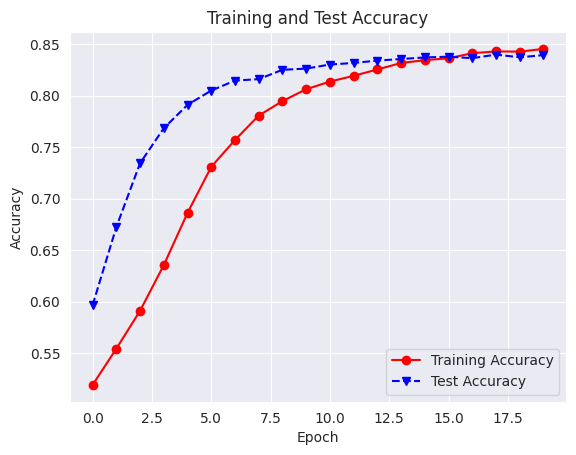
\includegraphics[width=0.50\textwidth]{Mlp_training_and_accuracy_plot}
	\caption{MLP training and test accuracy plot}\label{fig:mlp_training_and_accuracy_plot}
\end{figure}

A thorough analysis of the results reveals that the model maintains an accuracy of around 85\% throughout the epochs, indicating strong performance on the training data. In contrast, the test accuracy, though slightly lower than the training accuracy, remains stable around 80\% across epochs, suggesting reasonable generalization to unseen data. The observed gap between the training and test accuracy indicates potential overfitting, a common phenomenon where a model performs well on training data but struggles with unseen data.

\begin{figure}[H] 
	\centering
	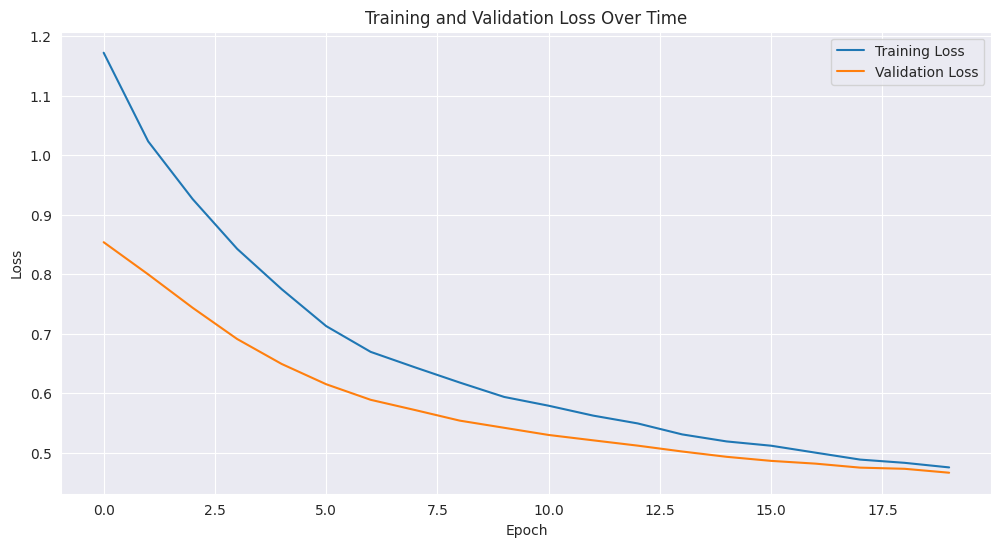
\includegraphics[width=0.50\textwidth]{Mlp_training_and_validation_loss_plot}
	\caption{MLP training and validation loss plot}\label{fig:mlp_training_and_validation_loss_plot}
\end{figure}

Additionally, the training and validation loss over time plot for this model shows a promising trend. It suggests that the model is learning effectively and avoiding overfitting. The training loss appears to be steadily decreasing over the epochs, indicating that the model is continually improving its ability to fit the training data. Similarly, the validation loss also shows a decreasing trend, although it fluctuates slightly more than the training loss. Overall, the validation loss follows a similar pattern to the training loss, indicating that the model is generalizing well and not overfitting to the training data.

\begin{figure}[H] 
	\centering
	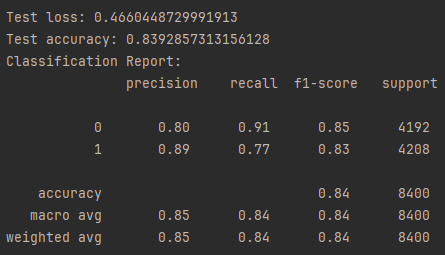
\includegraphics[width=0.50\textwidth]{Mlp_classification_report}
	\caption{Mlp training classification report}\label{fig:mlp_classification_report}
\end{figure}

% Overall performance of mlp %
The MLP model demonstrates strong performance on the test dataset, achieving an accuracy of 83.9\%. This accuracy reflects the model's ability to make correct predictions on unseen data. The precision, recall, and F1-score metrics provide a detailed assessment of the model's performance for each class. For class 0, the precision is 0.80, indicating that 80\% of the samples predicted as class 0 were correct, while the recall is 0.91, indicating that 91\% of the actual class 0 samples were identified correctly. Similarly, for class 1, the precision is 0.89 and the recall is 0.77. These metrics suggest that the model performs slightly better in identifying class 1 compared to class 0. The F1-scores for both classes are around 0.84, indicating a good balance between precision and recall. The classification report also includes macro and weighted average values, which provide a summarized view of the model's performance across both classes. The macro average values are 0.84 for all metrics, while the weighted average values are slightly higher at 0.85, reflecting a slight bias towards the slightly larger class (class 1). Overall, the classification report suggests that the MLP model generalizes well to unseen data and avoids overfitting, making it effective for the NLOS/LOS classification task.


\subsection{Comparison Between CNN and MLP}\label{cnn_vs_mlp}

% Decide whether are you using supervised or unsupervised learning? What algorithm should be preferred for your team? %
% Decide the split ratio of the training/test dataset such as 70:30 or 80:20? %
% Determine the classification, regression performance accuracy such as RMSE, confusion matrix etc? %
\subsection{Supervised Machine Learning Algorithms}\label{sml}

% TO WRITE %


% Decide whether are you using supervised or unsupervised learning? What algorithm should be preferred for your team? %
% Decide the split ratio of the training/test dataset such as 70:30 or 80:20? %
% Determine the classification, regression performance accuracy such as RMSE, confusion matrix etc? %
\subsection{Unsupervised Machine Learning Algorithms}\label{uml}


% TO WRITE %


% Plot the various performance indicators to illustrate the team choice and various result in data preprocessing & mining
\section{Data Visualization}\label{data_visualisation}

This section encompasses the graphical representation of data features and model architectures for enhanced comprehension.

\begin{description}[style=nextline]
    \item[Feature Visualization:] Visual depiction of both given and derived features for enhanced understanding.
    \item[Convolution Neural Network:] Visual representation of CNN model architecture to facilitate interpretation.
    \item[Multilayer Perceptron:] Visual depiction of MLP model architecture for improved insight into its workings.
\end{description}

\subsection{Feature Visualization}\label{feature_visualization}

\subsubsection{Frequency Graph of LOS and NLOS}\label{frequency_graph}

\begin{figure}[H] 
	\centering
	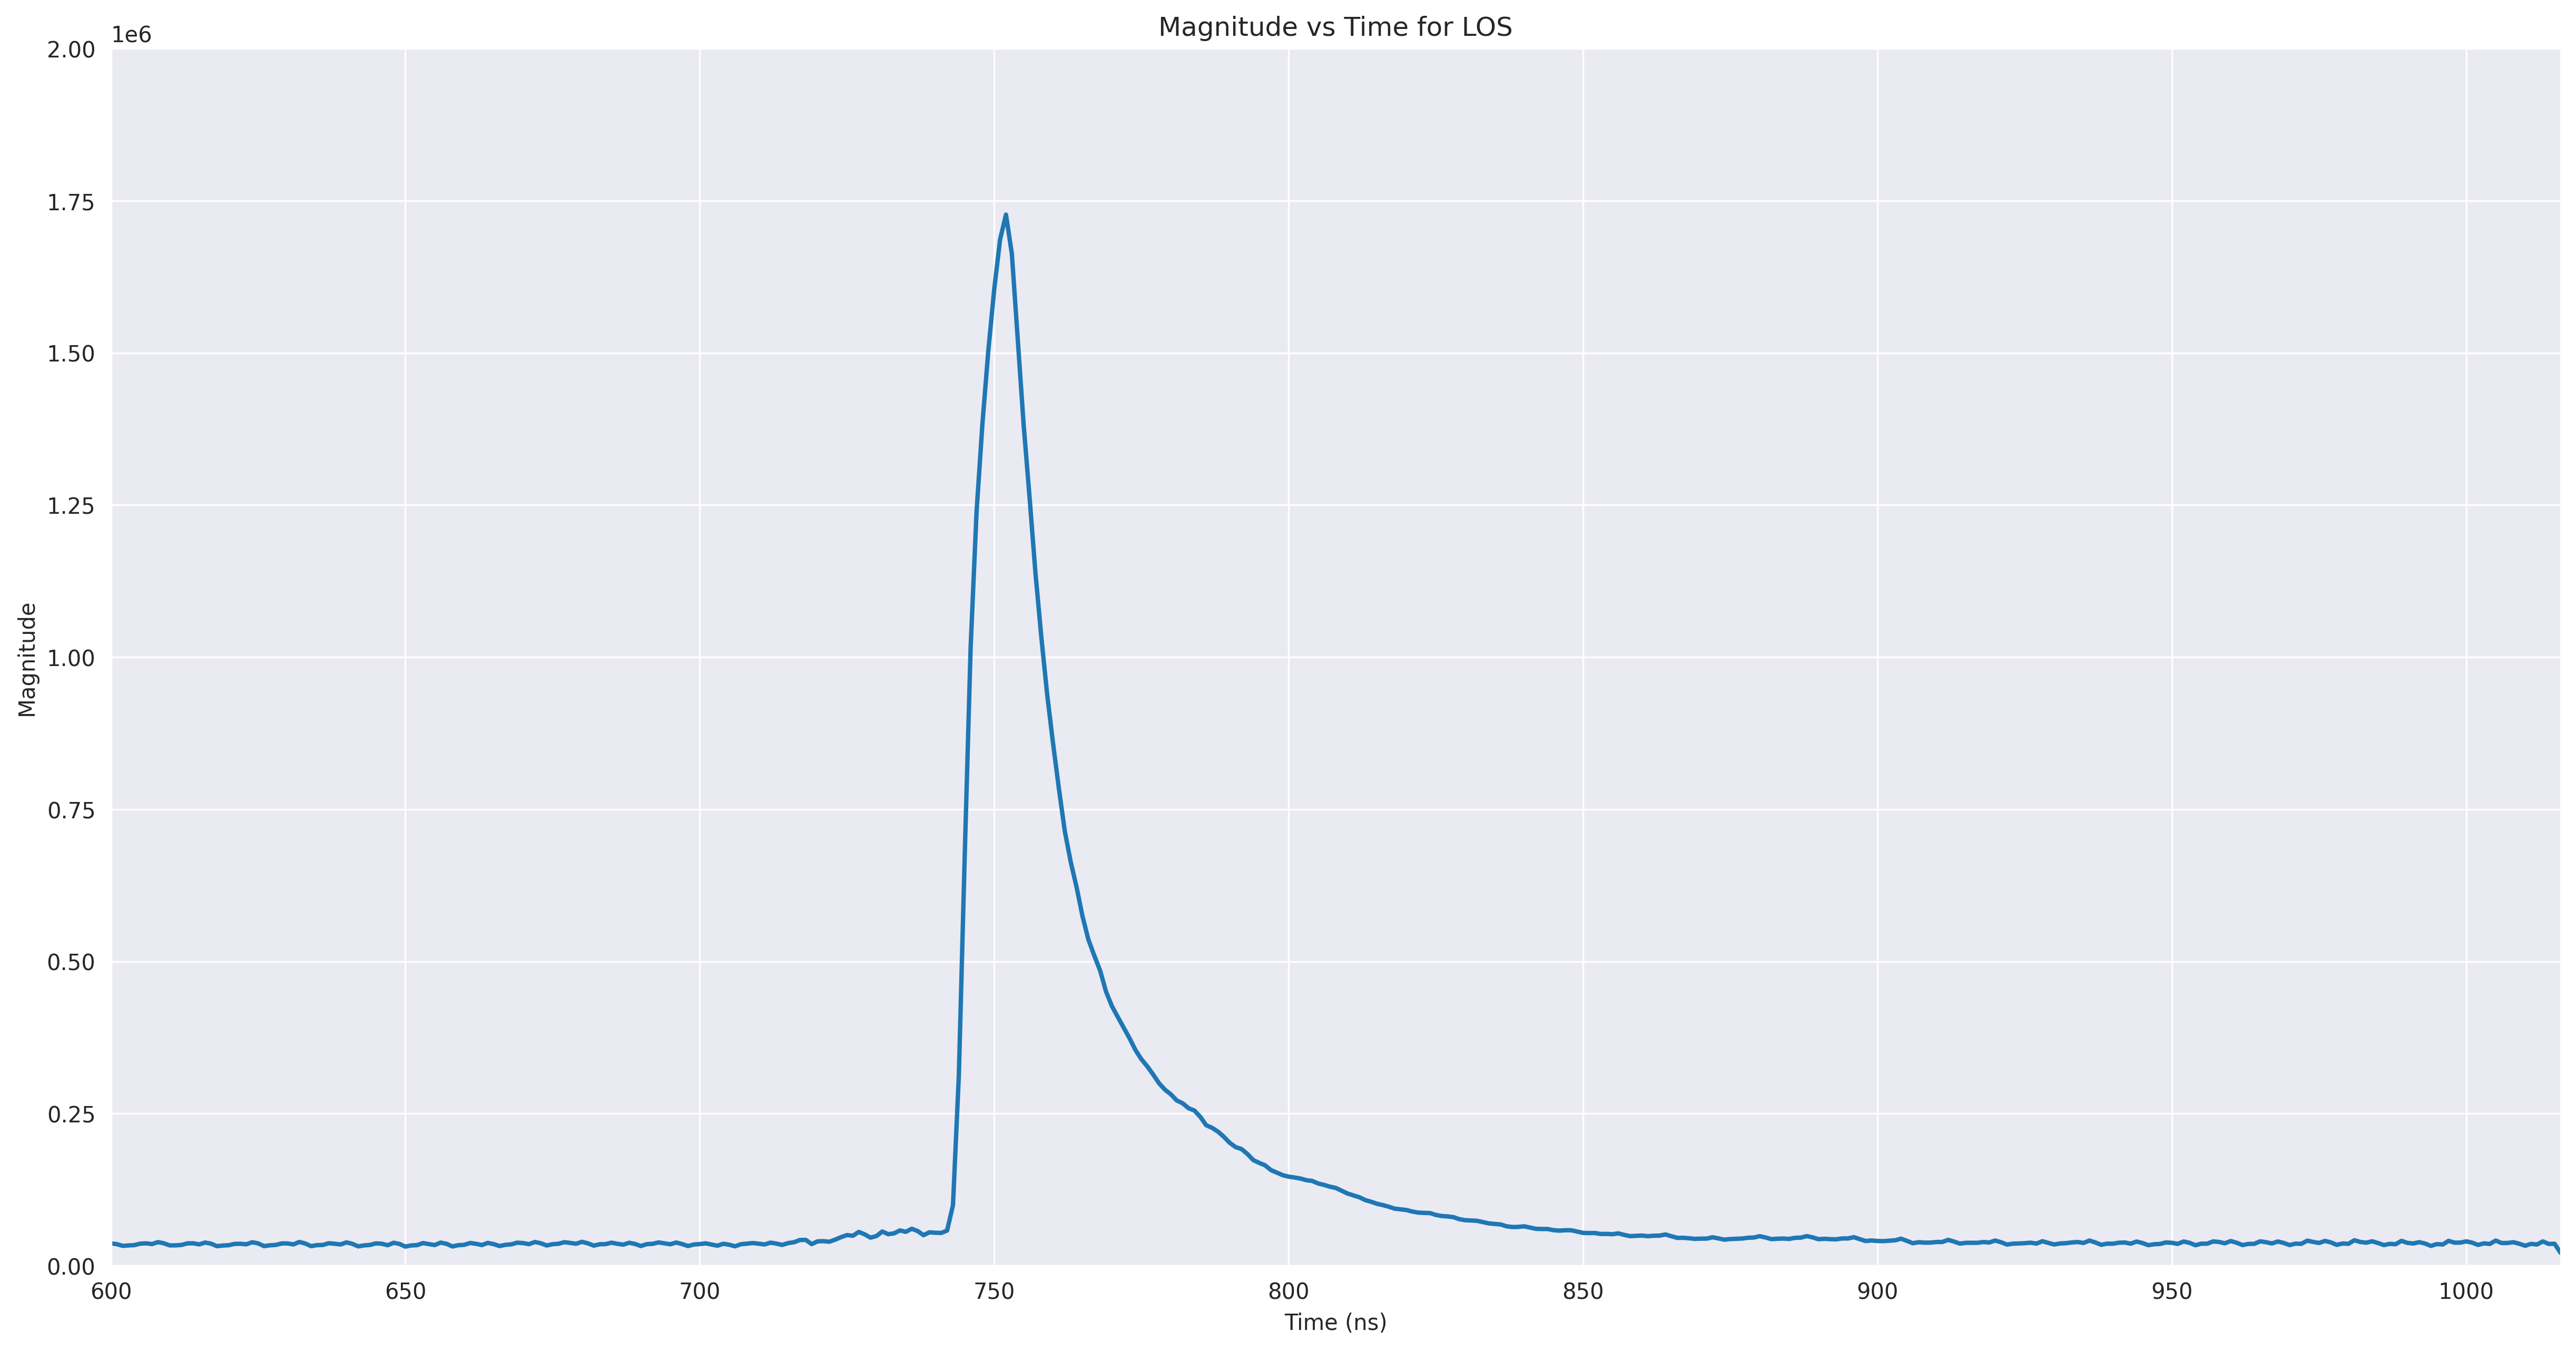
\includegraphics[width=0.50\textwidth]{LOS_Frequency_Graph.png}
	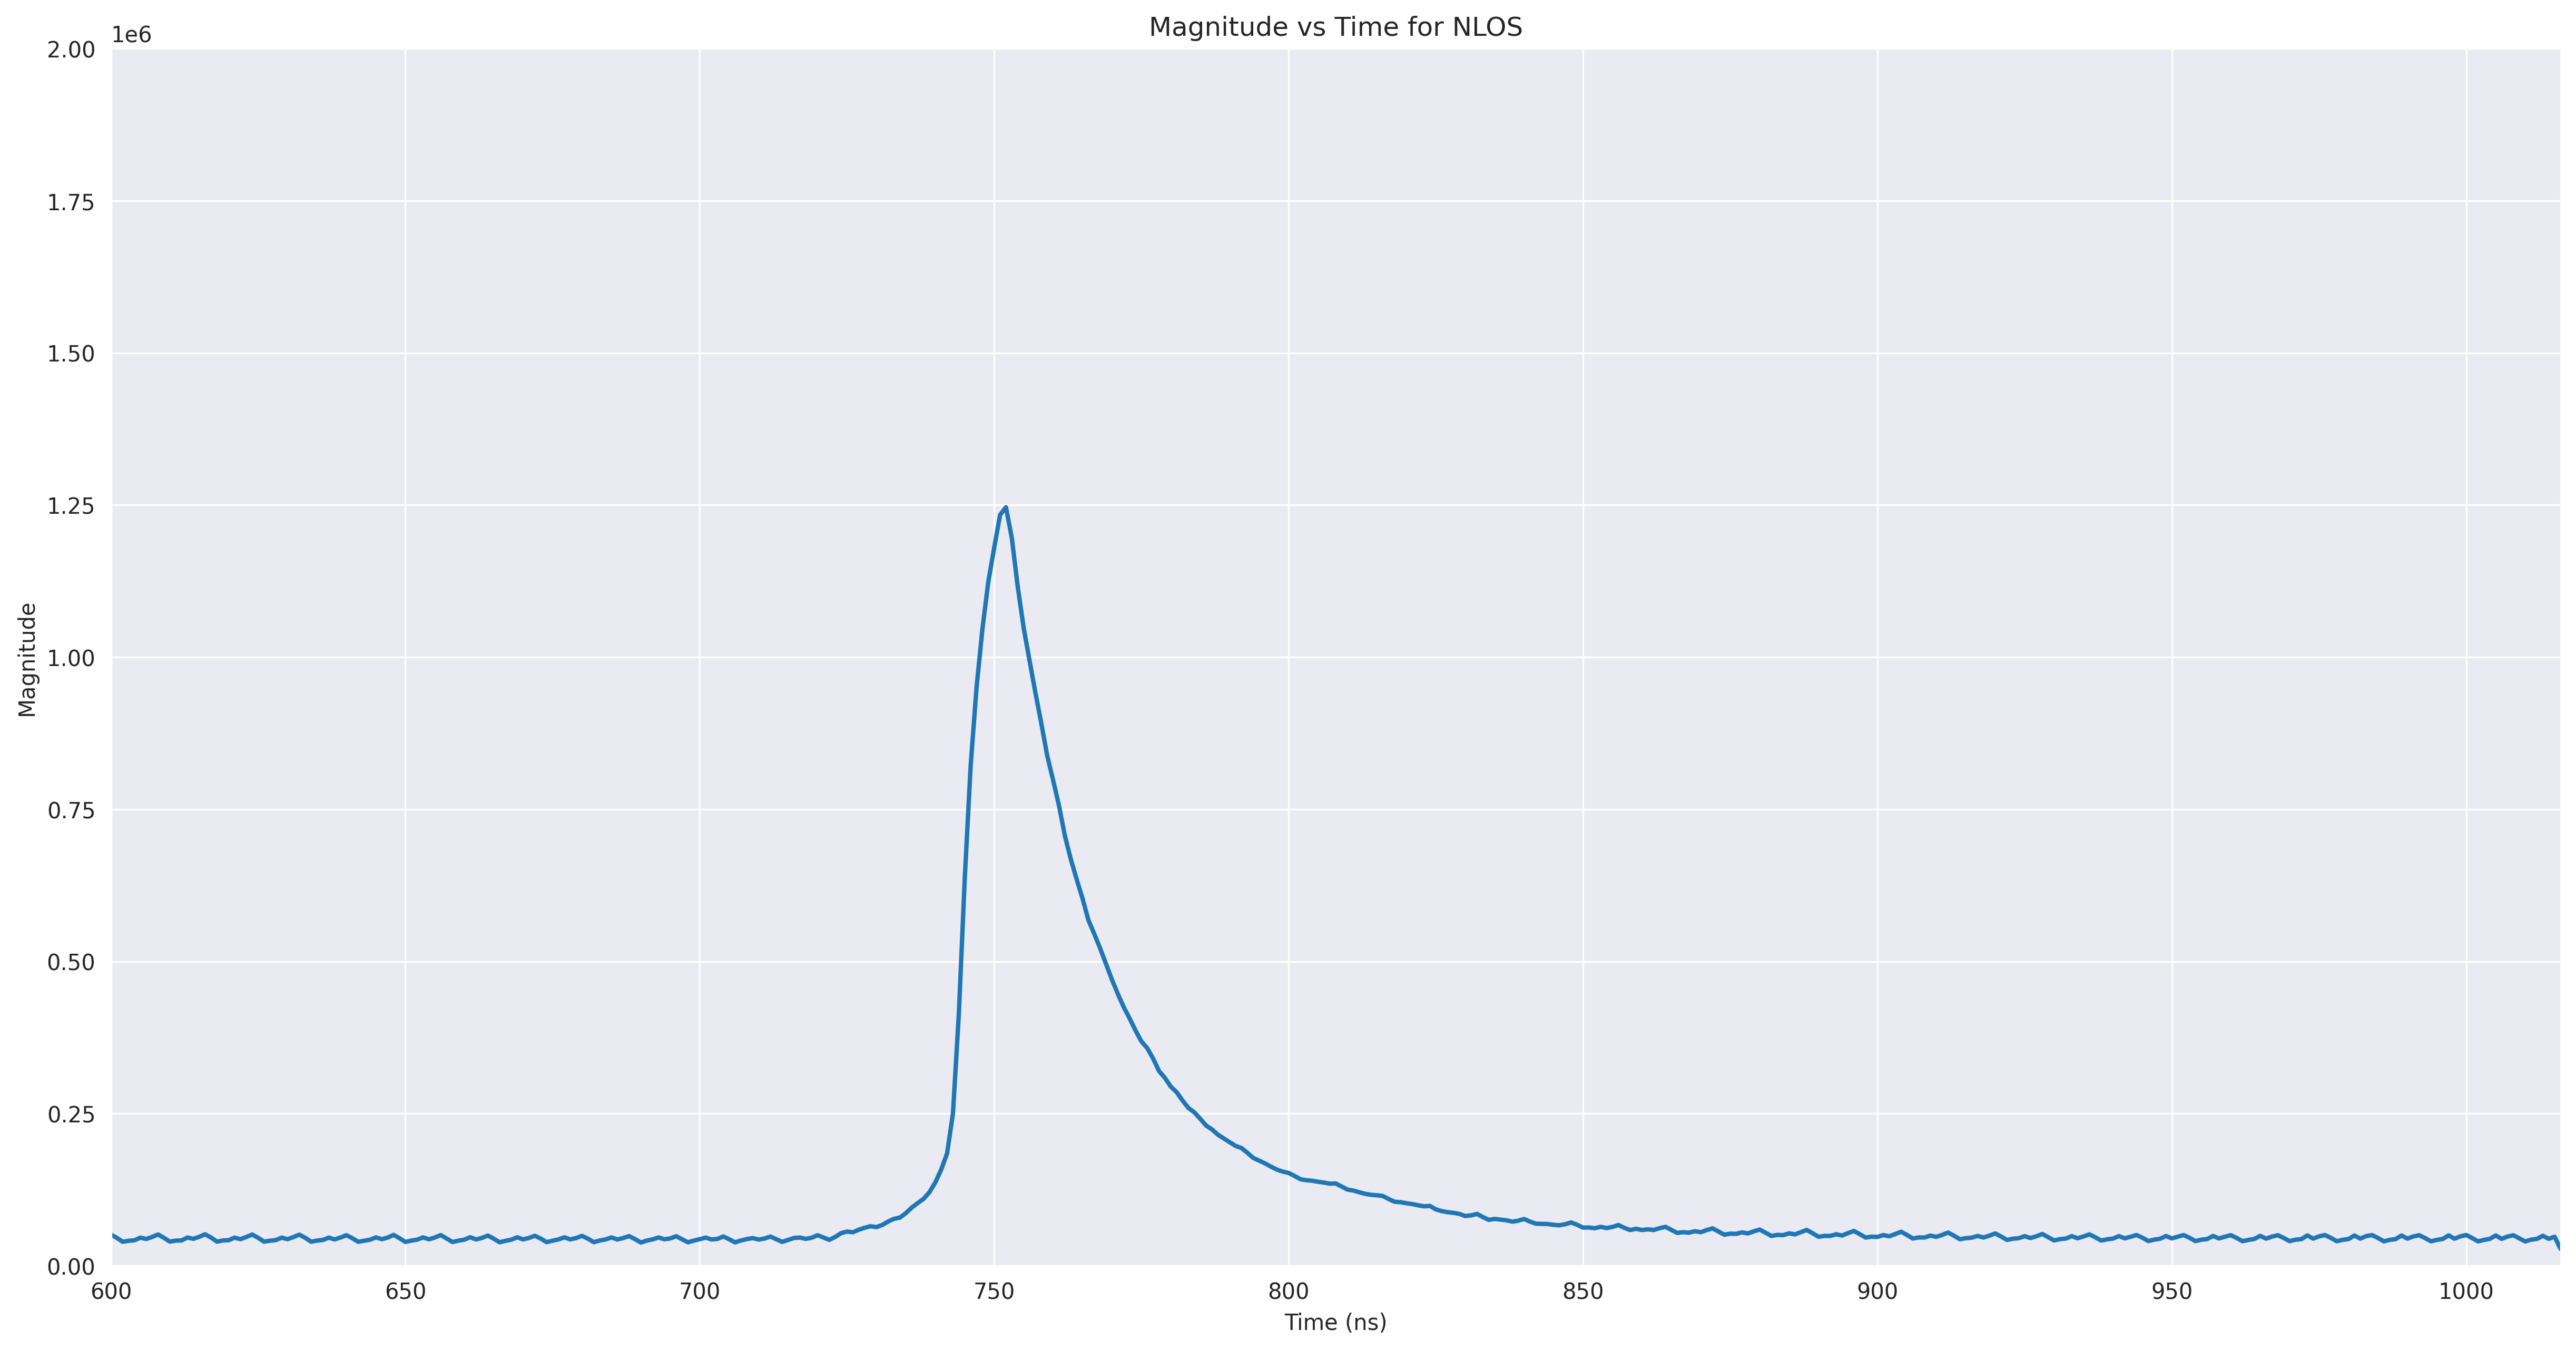
\includegraphics[width=0.50\textwidth]{NLOS_Frequency_Graph.png}
	\caption{Frequency Graph of LOS and NLOS}\label{fig:frequency_graph}
\end{figure}

\subsubsection{Frequency Graph of Wavelet Transformed LOS and NLOS}\label{frequency_graph_wavelet}

\begin{figure}[H] 
  \centering
  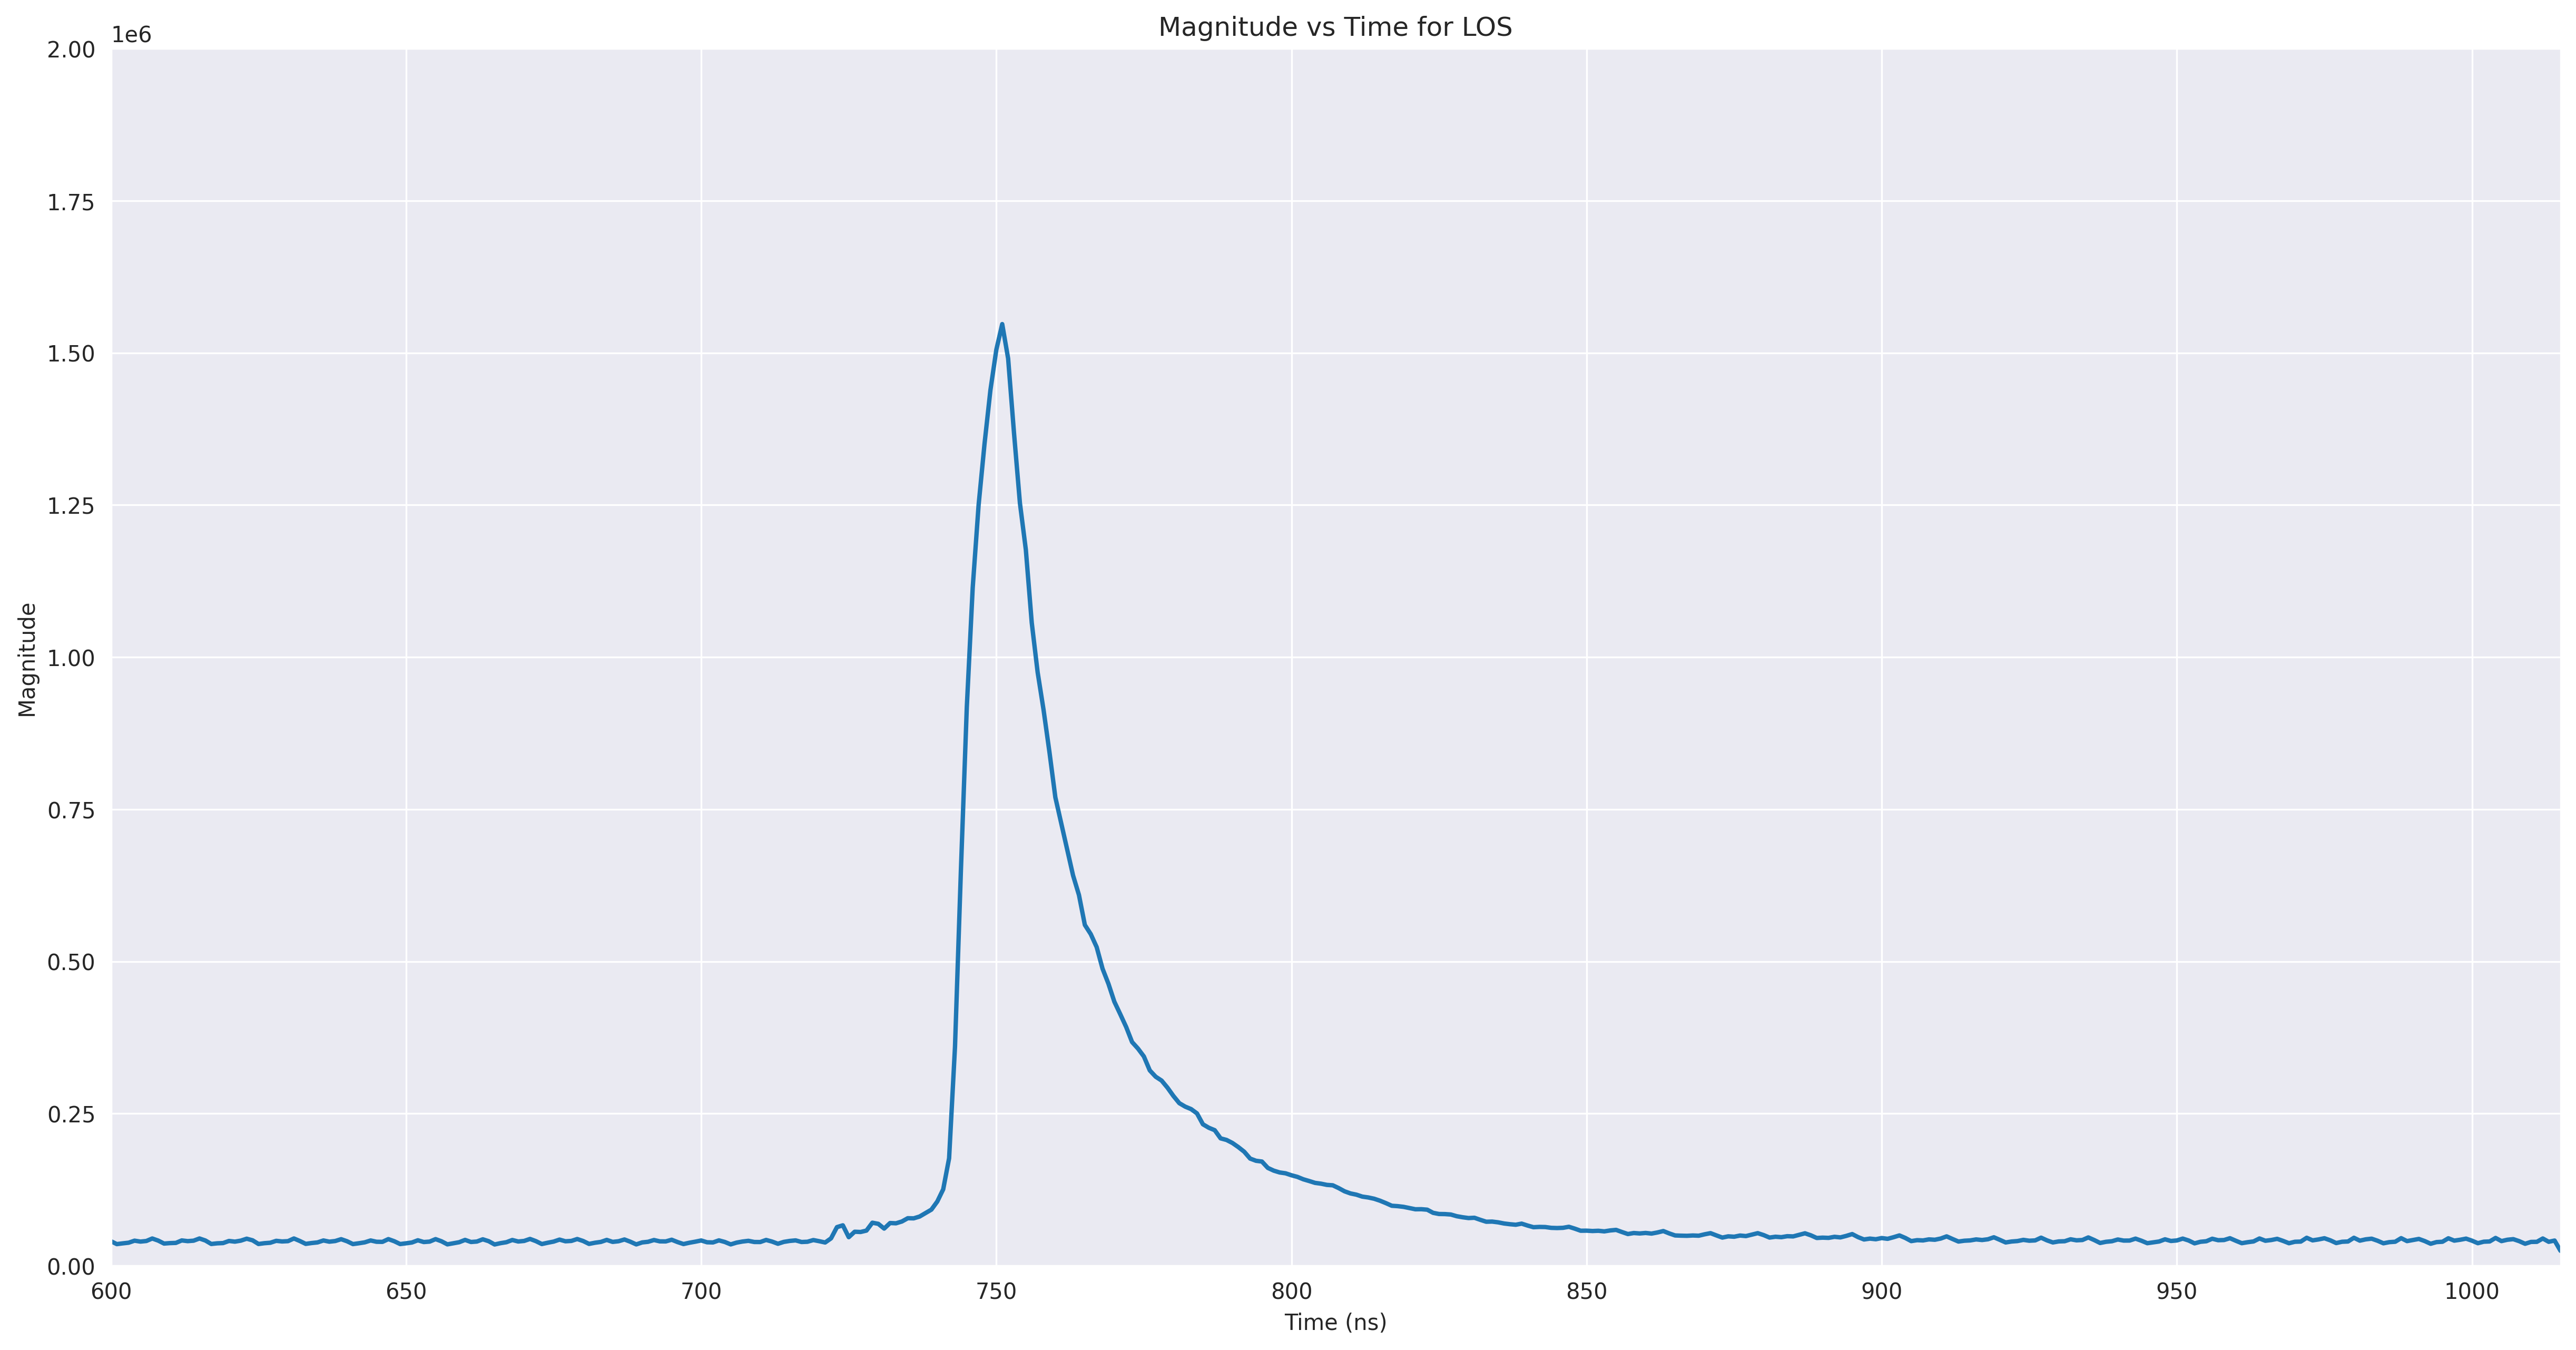
\includegraphics[width=0.50\textwidth]{Wavelet_Denoised_LOS_Frequency_Graph.png}
  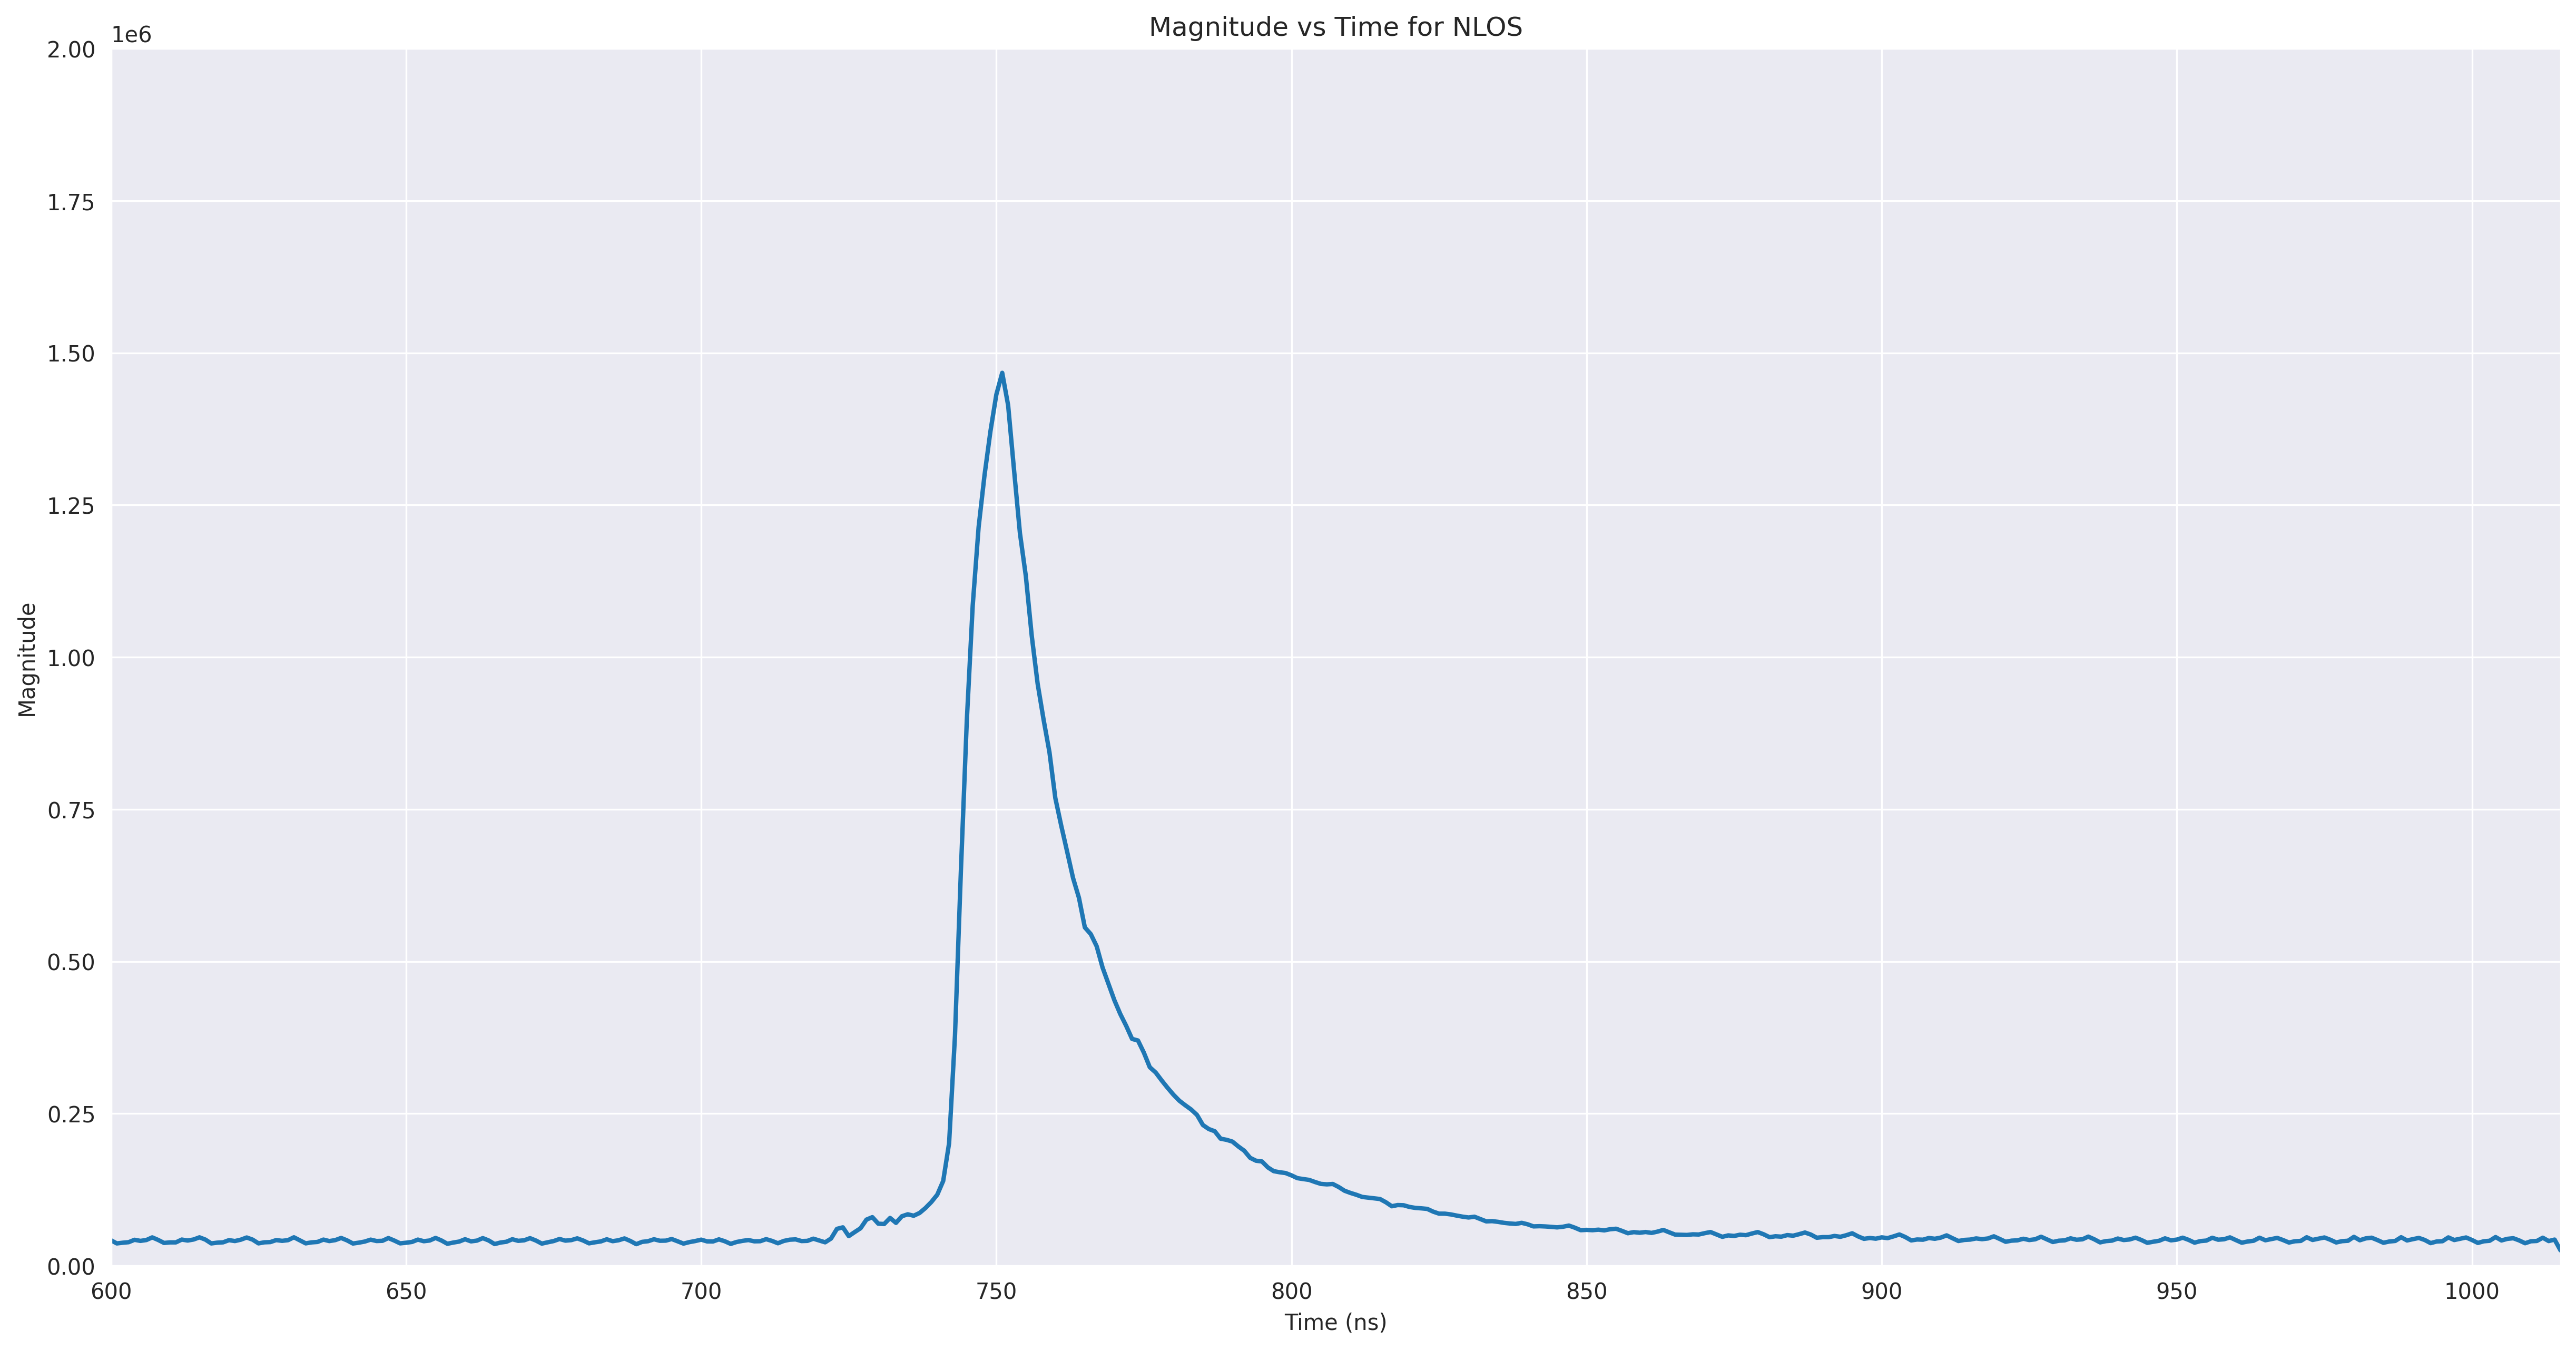
\includegraphics[width=0.50\textwidth]{Wavelet_Denoised_NLOS_Frequency_Graph.png}
  \caption{Frequency Graph of Wavelet Transformed LOS and NLOS}\label{fig:frequency_graph_wavelet}
\end{figure}

\subsubsection{Signal to Noise Raio}\label{sur_visual}

\begin{figure}[H] % [H] forces the figure to be placed exactly where it appears in the text
	\centering % Horizontally center the figure
	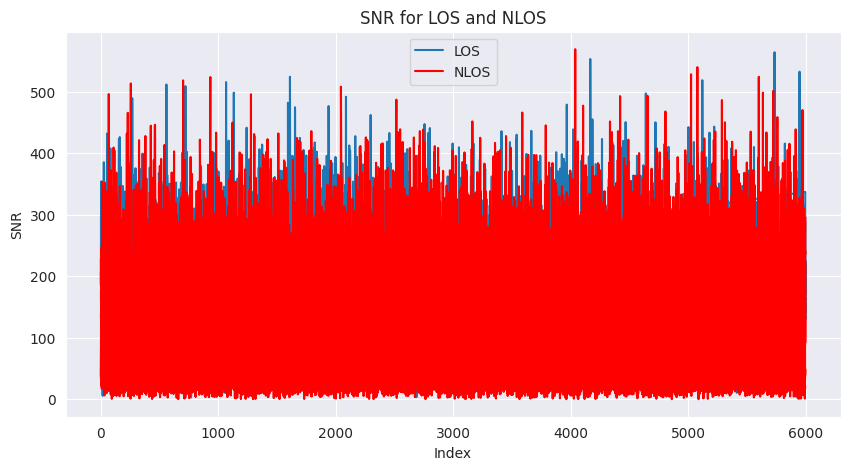
\includegraphics[width=0.65\textwidth]{SNR} % Include the figure
	\caption{Signal to Noise Ratio}\label{fig:snr}
\end{figure}


\subsection{Convolution Neural Network}\label{cnn_visual}

\subsection{Multilayer Perceptron}\label{mlp_visual}


% \begin{center}
% 	\begin{tabular}{l r}
% 		Date Performed: & February 13, 2022 \\ % Date the experiment was performed
% 		Partners: & Cecilia \textsc{Smith} \\ % Partner names
% 		& Tajel \textsc{Khumalo} \\
% 		Instructor: & Professor \textsc{Rivera} % Instructor/supervisor
% 	\end{tabular}
% \end{center}

% If you need to include an abstract, uncomment the lines below
%\begin{abstract}
%	Abstract text
%\end{abstract}

%----------------------------------------------------------------------------------------
%	OBJECTIVE
%----------------------------------------------------------------------------------------

% \section{Objective}





% To determine the atomic weight of magnesium via its reaction with oxygen and to study the stoichiometry of the reaction (as defined in \ref{definitions}):

% \begin{center}
% 	\ce{2 Mg + O2 -> 2 MgO} % Chemical equations entered in \ce{} commands, see the mhchem package documentation for more information
% \end{center}

% If you have more than one objective, uncomment the below:
%\begin{description}
%	\item[First Objective] \hfill \\
%	Objective 1 text
%	\item[Second Objective] \hfill \\
%	Objective 2 text
%\end{description}

% \begin{description}
% 	\item[Stoichiometry] The relationship between the relative quantities of substances taking part in a reaction or forming a compound, typically a ratio of whole integers.
% 	\item[Atomic mass] The mass of an atom of a chemical element expressed in atomic mass units. It is approximately equivalent to the number of protons and neutrons in the atom (the mass number) or to the average number allowing for the relative abundances of different isotopes. 
% \end{description} 
 
%----------------------------------------------------------------------------------------
%	EXPERIMENTAL DATA
%----------------------------------------------------------------------------------------

% \section{Experimental Data}

% \begin{tabular}{l l}
% 	Mass of empty crucible & \SI{7.28}{\gram}\\ % Scientific/technical units are output using the \SI command, see the siunitx package documentation for more information on how to use this command
% 	Mass of crucible and magnesium before heating & \SI{8.59}{\gram}\\
% 	Mass of crucible and magnesium oxide after heating & \SI{9.46}{\gram}\\
% 	Balance used & \#4\\
% 	Magnesium from sample bottle & \#1
% \end{tabular}

%----------------------------------------------------------------------------------------
%	SAMPLE CALCULATION
%----------------------------------------------------------------------------------------

% \section{Sample Calculation}

% \begin{tabular}{ll}
% 	Mass of magnesium metal & = \SI{8.59}{\gram} - \SI{7.28}{\gram}\\
% 	& = \SI{1.31}{\gram}\\
% 	Mass of magnesium oxide & = \SI{9.46}{\gram} - \SI{7.28}{\gram}\\
% 	& = \SI{2.18}{\gram}\\
% 	Mass of oxygen & = \SI{2.18}{\gram} - \SI{1.31}{\gram}\\
% 	& = \SI{0.87}{\gram}
% \end{tabular}

% Because of this reaction, the required ratio is the atomic weight of magnesium: \SI{16.00}{\gram} of oxygen as experimental mass of Mg: experimental mass of oxygen or $\frac{x}{1.31} = \frac{16}{0.87}$ from which, $M_{\ce{Mg}} = 16.00 \times \frac{1.31}{0.87} = 24.1 = \SI{24}{\gram\per\mole}$ (to two significant figures).

%----------------------------------------------------------------------------------------
%	RESULTS AND CONCLUSIONS
%----------------------------------------------------------------------------------------

% \section{Results and Conclusions}

% The atomic weight of magnesium is concluded to be \SI{24}{\gram\per\mol}, as determined by the stoichiometry of its chemical combination with oxygen. This result is in agreement with the accepted value.

% \begin{figure}[H] % [H] forces the figure to be placed exactly where it appears in the text
% 	\centering % Horizontally center the figure
% 	
\includegraphics[width=0.65\textwidth]{placeholder} % Include the figure
% 	\caption{Figure caption.}
% \end{figure}

%----------------------------------------------------------------------------------------
%	DISCUSSION
%----------------------------------------------------------------------------------------

% \section{Discussion of Experimental Uncertainty}

% The accepted value (periodic table) is \SI{24.3}{\gram\per\mole} \autocite{Smith:2022qr}. The percentage discrepancy between the accepted value and the result obtained here is 1.3\%. Because only a single measurement was made, it is not possible to calculate an estimated standard deviation (see \textcite{Smith:2021jd}).
 
% The most obvious source of experimental uncertainty is the limited precision of the balance. Other potential sources of experimental uncertainty are: the reaction might not be complete; if not enough time was allowed for total oxidation, less than complete oxidation of the magnesium might have, in part, reacted with nitrogen in the air (incorrect reaction); the magnesium oxide might have absorbed water from the air, and thus weigh ``too much." Because the result obtained is close to the accepted value it is possible that some of these experimental uncertainties have fortuitously cancelled one another.

%----------------------------------------------------------------------------------------
%	ANSWERS TO DEFINITIONS
%----------------------------------------------------------------------------------------

% \section{Answers to Definitions}

% \begin{enumerate}
% 	\item The \textit{atomic weight of an element} is the relative weight of one of its atoms compared to C-12 with a weight of 12.0000000$\ldots$, hydrogen with a weight of 1.008, to oxygen with a weight of 16.00. Atomic weight is also the average weight of all the atoms of that element as they occur in nature.
% 	\item The \textit{units of atomic weight} are two-fold, with an identical numerical value. They are g/mole of atoms (or just g/mol) or amu/atom.
% 	\item \textit{Percentage discrepancy} between an accepted (literature) value and an experimental value is:
% 		\begin{equation*}
% 			\frac{\mathrm{experimental\;result} - \mathrm{accepted\;result}}{\mathrm{accepted\;result}}
% 		\end{equation*}
% \end{enumerate}

%----------------------------------------------------------------------------------------
%	BIBLIOGRAPHY
%----------------------------------------------------------------------------------------

\printbibliography % Output the bibliography

%----------------------------------------------------------------------------------------

\end{document}
